

\subsection{Qualitative Data}
\par
In the dynamic landscape of stock markets, fundamental analysis plays a pivotal role in understanding the nuances of stock performance. This report delves into the qualitative aspects of the LQ45 index companies, focusing on the categorization of these entities into state-owned and private-owned enterprises from 2017 to 2021.

\begin{table}[H]
    \centering
    
    \caption{Type of the company listed in LQ45 2017 - 2021}
    
    \centering
    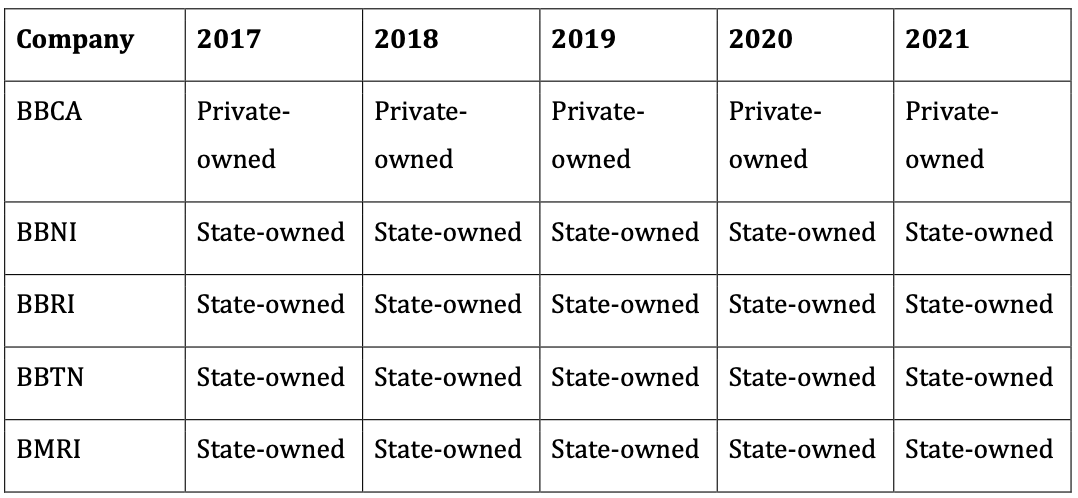
\includegraphics[width = 0.8\textwidth]{figures/table_1.png}
    \label{tab:}
\end{table}

\paragraph{Conclusion:}
\par The qualitative analysis of the LQ45 index companies underscores the enduring dominance of state-owned enterprises and the consequential implications for stock performance. By delving into ownership structures and profitability dynamics, this report provides valuable insights for investors, policymakers, and stakeholders navigating the complexities of the stock market.

\subsection{Quantitative Data}

This section delves into the quantitative data derived from monthly closing stock prices of prominent companies within the LQ45 index, namely BBCA, BBNI, BBRI, BBTN, and BMRI. Through the calculation of monthly stock returns, we unravel the patterns and trends shaping the investment landscape.

Data used in this report is in the form of monthly closing stock prices which are then processed to obtain the monthly stock returns of BBCA, BBNI, BBRI, BBTN, and BMRI using the formula:

$$
\text{Return}_{t} = \frac{\text{Closing Price}_{t} - \text{Closing Price}_{t-1}}{\text{Closing Price}_{t-1}}
$$

\begin{figure}[H]
    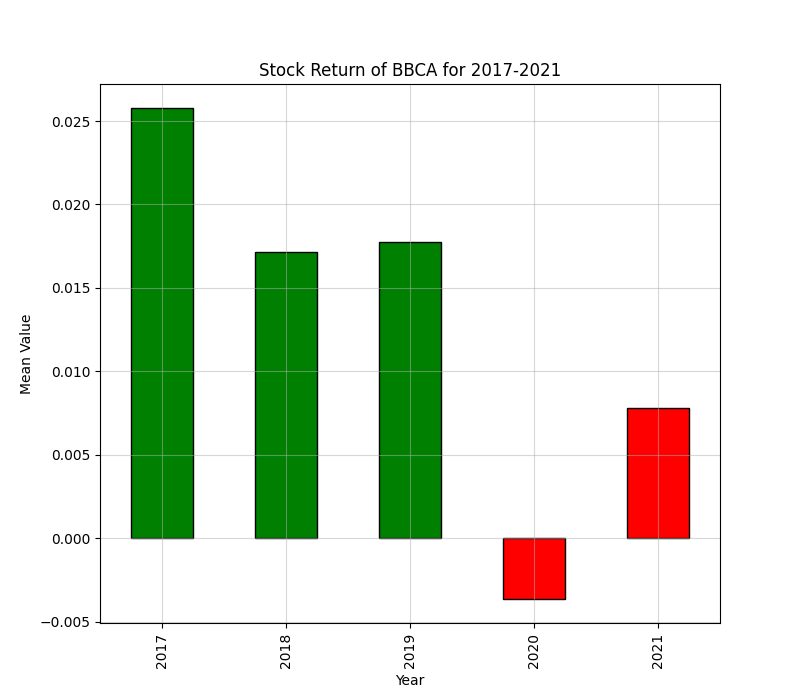
\includegraphics[width = .55\textwidth ]{figures/BBCA.png}
    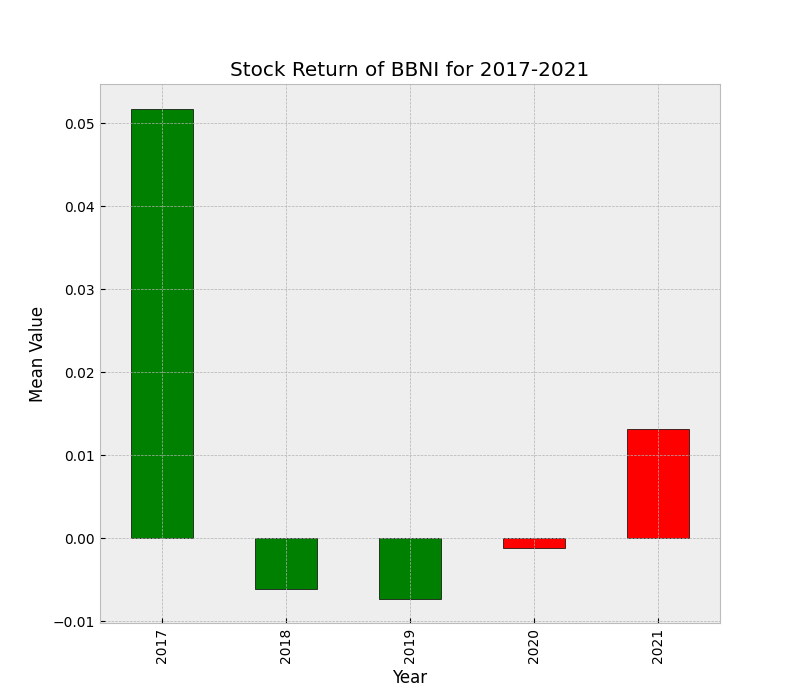
\includegraphics[width = .55\textwidth ]{figures/BBNI.png}
\end{figure}

\begin{figure}[H]
    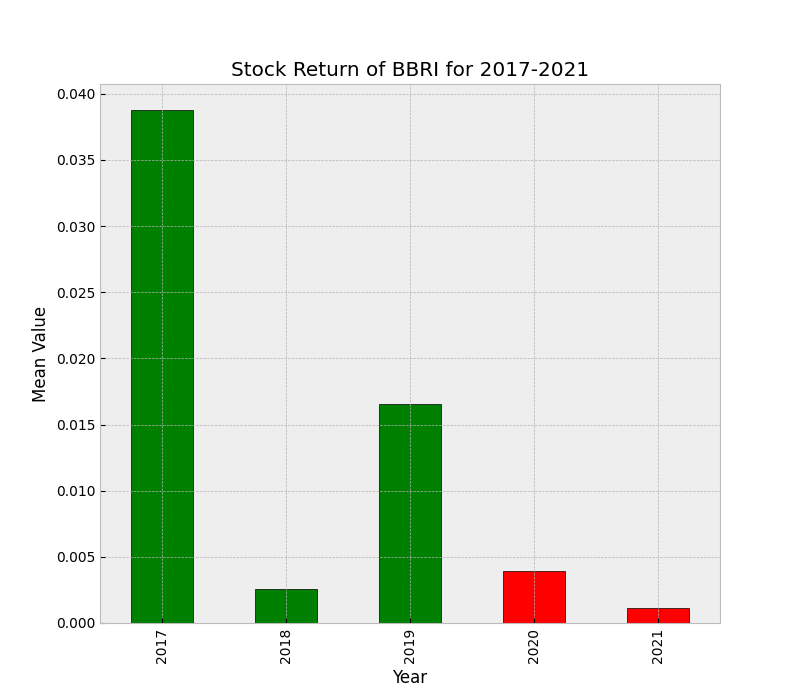
\includegraphics[width = .55\textwidth ]{figures/BBRI.png}
    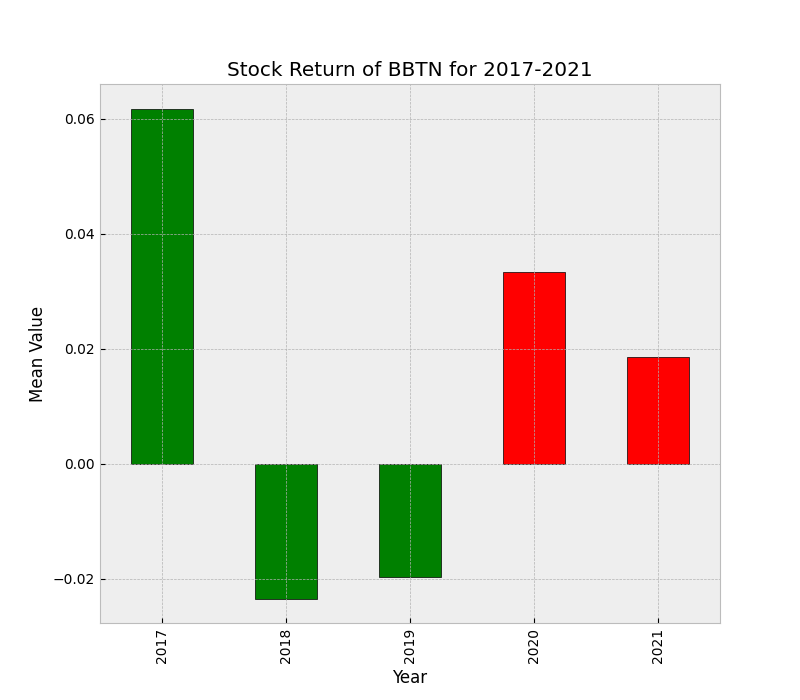
\includegraphics[width = .55\textwidth ]{figures/BBTN.png}
\end{figure}

\begin{figure}[H]
    \centering
    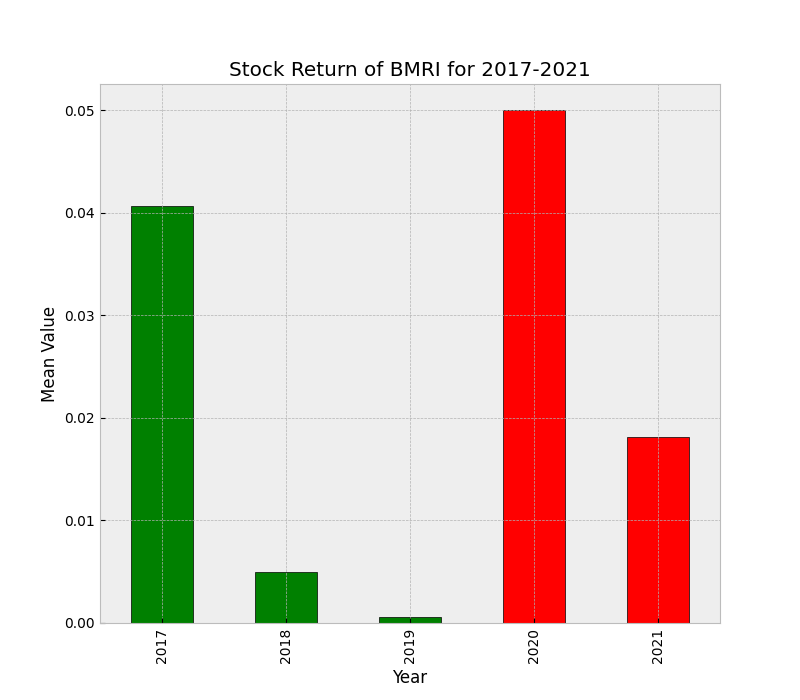
\includegraphics[width = .55\textwidth ]{figures/BMRI.png}
\end{figure}

\paragraph{Conclusion:}
\par The quantitative analysis of monthly stock returns provides valuable insights into the performance dynamics of selected companies within the LQ45 index. By leveraging quantitative data, investors can make informed decisions, optimize investment strategies, and navigate the complexities of the stock market with confidence.







